%% figuras.tex
%% Todas as figuras do relatório. Cada figura é um comando usado no ponto
%% certo de relatorio-mt-duas-fitas.tex (carregado com %% figuras.tex
%% Todas as figuras do relatório. Cada figura é um comando usado no ponto
%% certo de relatorio-mt-duas-fitas.tex (carregado com %% figuras.tex
%% Todas as figuras do relatório. Cada figura é um comando usado no ponto
%% certo de relatorio-mt-duas-fitas.tex (carregado com %% figuras.tex
%% Todas as figuras do relatório. Cada figura é um comando usado no ponto
%% certo de relatorio-mt-duas-fitas.tex (carregado com \input{figuras}).
%%
%% Organização da pasta figuras/:
%%   figuras/diagramas/   diagramas de transição (completo e por bloco)
%%   figuras/resumo.png   tabela final dos 9 testes
%%   figuras/execucao/    passo a passo de cada teste (testeN_PP.png)
%%
%% figuras/resumo.png e figuras/execucao/ foram geradas pelo simulador da
%% pasta MaquinaDeTuring (função salvar_imagens, 48 linhas por página):
%%   python3 mt_duas_fitas.py --resumo --imagem figuras/resumo.png
%% O passo a passo de cada teste (na ordem da lista TESTES) foi salvo sem a
%% tabela de resumo no final, como figuras/execucao/testeN_PP.png.

% ======================================================================
% Capítulo 1 -- Diagramas de transição
% ======================================================================

\newcommand{\FiguraDiagramaCompleto}{%
\begin{figure}[H]
\centering
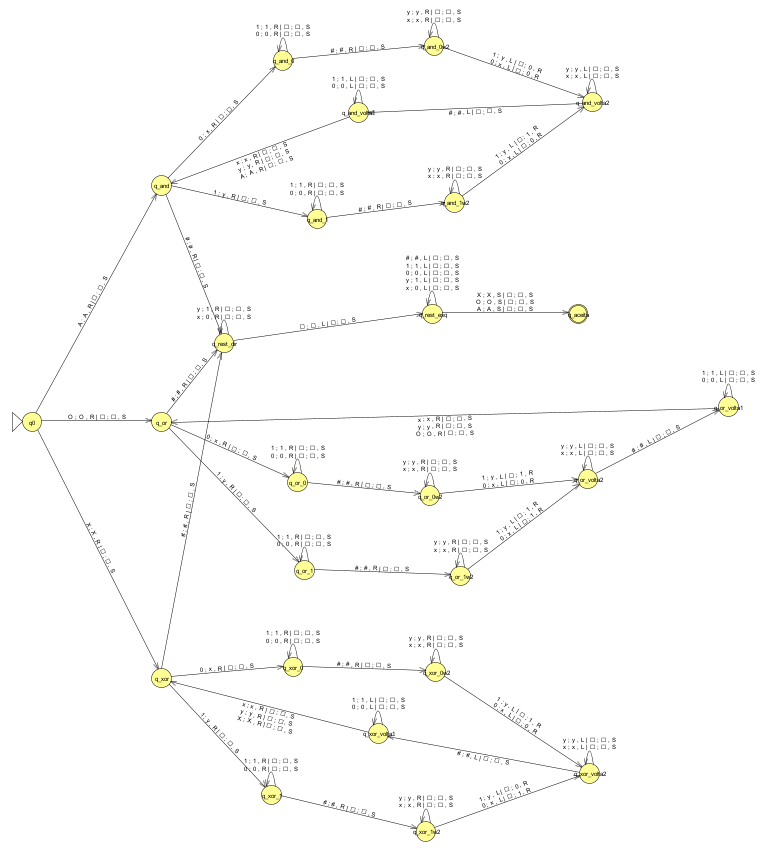
\includegraphics[width=\linewidth,height=0.72\textheight,keepaspectratio]{figuras/diagramas/diag_completo.png}
\caption{Diagrama completo da máquina (25 estados, 89 transições)}
\label{fig:diagrama}
\end{figure}}

\newcommand{\FiguraBlocos}{%
\begin{figure}[H]
\centering
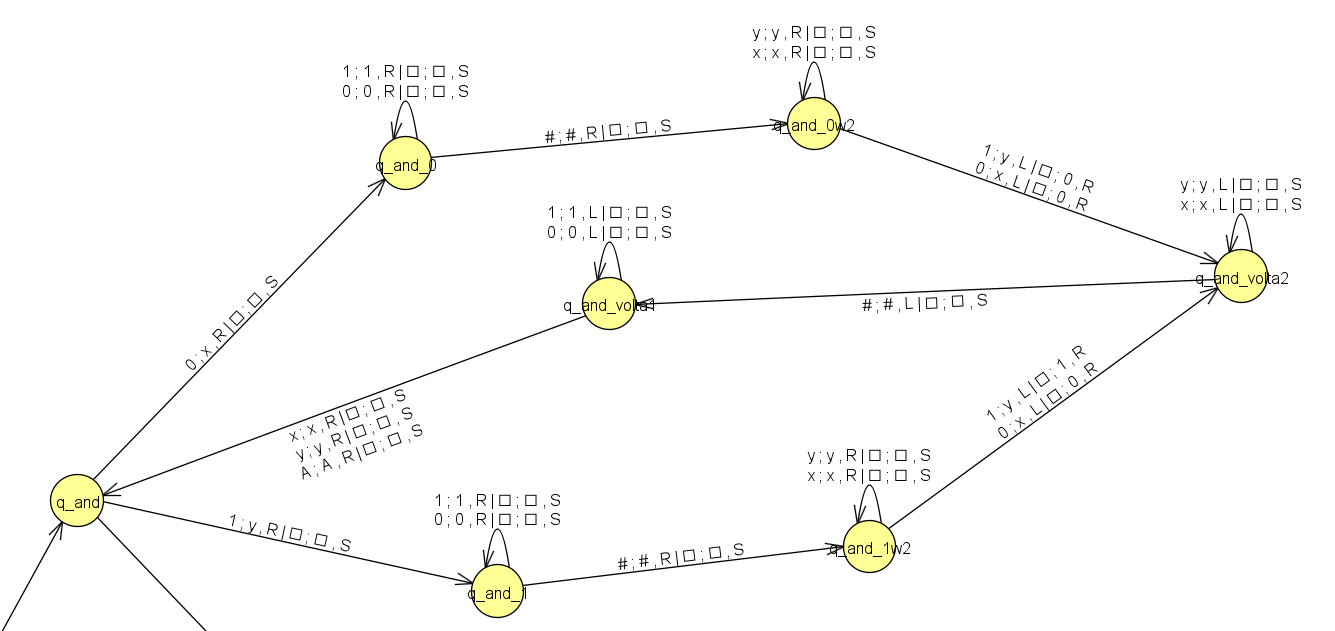
\includegraphics[width=\linewidth,height=0.22\textheight,keepaspectratio]{figuras/diagramas/diag_and.png}\\[0.2em]
{\small (a) Bloco AND}\\[0.8em]
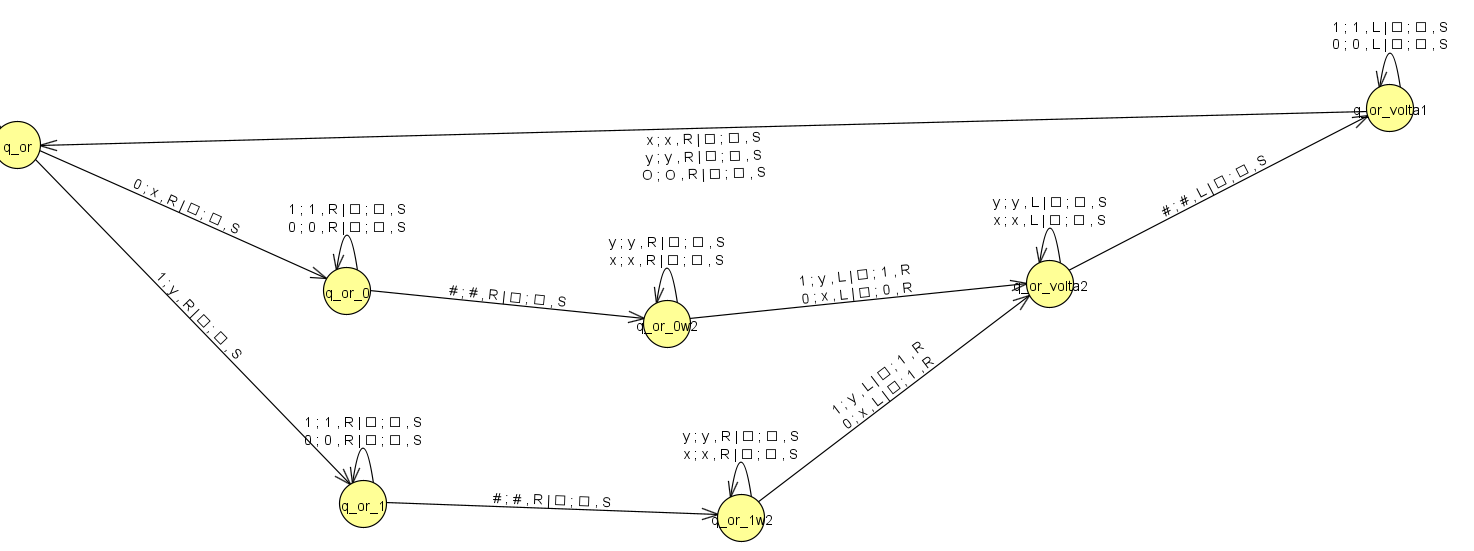
\includegraphics[width=\linewidth,height=0.22\textheight,keepaspectratio]{figuras/diagramas/diag_or.png}\\[0.2em]
{\small (b) Bloco OR}\\[0.8em]
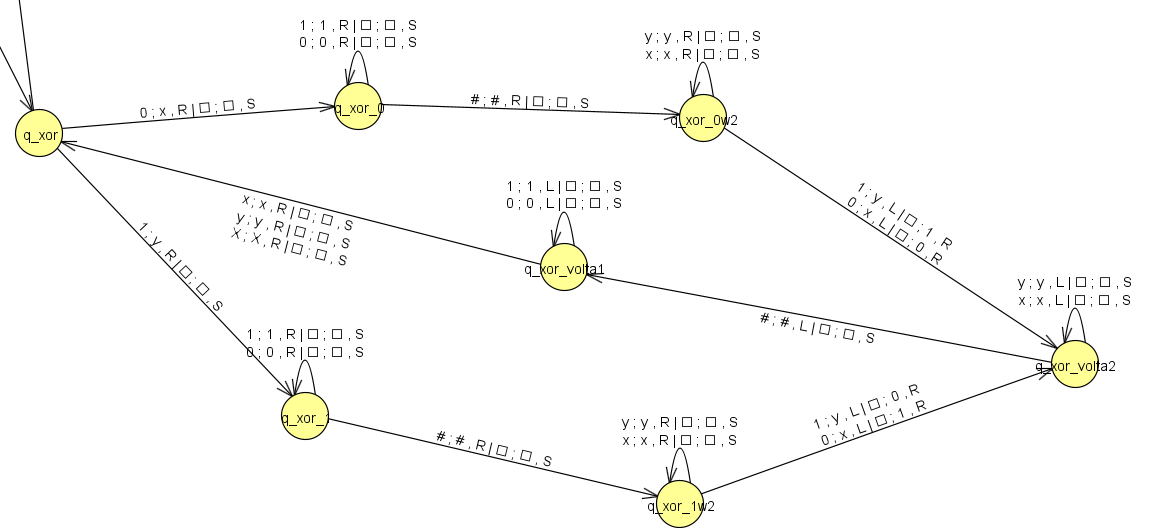
\includegraphics[width=\linewidth,height=0.22\textheight,keepaspectratio]{figuras/diagramas/diag_xor.png}\\[0.2em]
{\small (c) Bloco XOR}
\caption{Ampliação de cada bloco de operação}
\label{fig:blocos}
\end{figure}}

% ======================================================================
% Capítulo 3 -- Resumo dos testes
% ======================================================================

\newcommand{\FiguraResumo}{%
\begin{figure}[H]
\centering
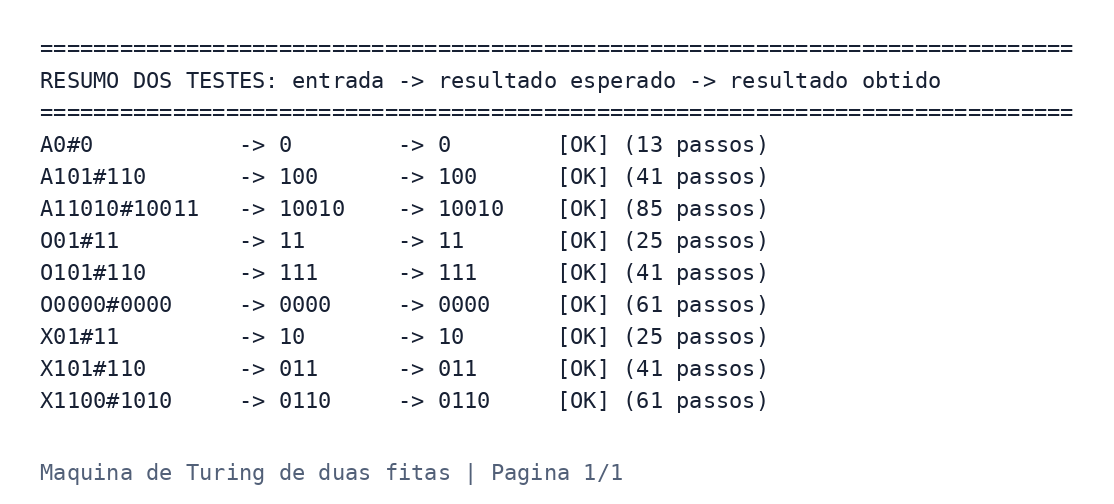
\includegraphics[width=\linewidth]{figuras/resumo.png}
\caption{Resumo da execução dos testes}
\label{fig:resumo}
\end{figure}}

% ======================================================================
% Capítulo 3 -- Execução passo a passo
% ======================================================================

% \PaginaExecucao{arquivo}{entrada}{esperado}{parte}{total}
\newcommand{\PaginaExecucao}[5]{%
\begin{figure}[H]
\centering
\includegraphics[width=\linewidth,height=0.78\textheight,keepaspectratio]{figuras/execucao/#1.png}
\caption{Execução passo a passo da entrada \texttt{#2} (esperado: \texttt{#3})\ifnum#5>1\ --- parte #4 de #5\fi}
\end{figure}}

\newcommand{\FigurasExecucao}{%

% ── Teste 1: A0#0 → 0 (13 passos) ─────────────────────────────────────
\subsection{Teste 1: \texttt{A0\#0}}
\label{sec:teste1}
\PaginaExecucao{teste1_01}{A0\#0}{0}{1}{1}

% ── Teste 2: A101#110 → 100 (41 passos) ───────────────────────────────
\subsection{Teste 2: \texttt{A101\#110}}
\label{sec:teste2}
\PaginaExecucao{teste2_01}{A101\#110}{100}{1}{3}
\PaginaExecucao{teste2_02}{A101\#110}{100}{2}{3}
\PaginaExecucao{teste2_03}{A101\#110}{100}{3}{3}

% ── Teste 3: A11010#10011 → 10010 (85 passos) ─────────────────────────
\subsection{Teste 3: \texttt{A11010\#10011}}
\label{sec:teste3}
\PaginaExecucao{teste3_01}{A11010\#10011}{10010}{1}{6}
\PaginaExecucao{teste3_02}{A11010\#10011}{10010}{2}{6}
\PaginaExecucao{teste3_03}{A11010\#10011}{10010}{3}{6}
\PaginaExecucao{teste3_04}{A11010\#10011}{10010}{4}{6}
\PaginaExecucao{teste3_05}{A11010\#10011}{10010}{5}{6}
\PaginaExecucao{teste3_06}{A11010\#10011}{10010}{6}{6}

% ── Teste 4: O01#11 → 11 (25 passos) ──────────────────────────────────
\subsection{Teste 4: \texttt{O01\#11}}
\label{sec:teste4}
\PaginaExecucao{teste4_01}{O01\#11}{11}{1}{2}
\PaginaExecucao{teste4_02}{O01\#11}{11}{2}{2}

% ── Teste 5: O101#110 → 111 (41 passos) ───────────────────────────────
\subsection{Teste 5: \texttt{O101\#110}}
\label{sec:teste5}
\PaginaExecucao{teste5_01}{O101\#110}{111}{1}{3}
\PaginaExecucao{teste5_02}{O101\#110}{111}{2}{3}
\PaginaExecucao{teste5_03}{O101\#110}{111}{3}{3}

% ── Teste 6: O0000#0000 → 0000 (61 passos) ────────────────────────────
\subsection{Teste 6: \texttt{O0000\#0000}}
\label{sec:teste6}
\PaginaExecucao{teste6_01}{O0000\#0000}{0000}{1}{4}
\PaginaExecucao{teste6_02}{O0000\#0000}{0000}{2}{4}
\PaginaExecucao{teste6_03}{O0000\#0000}{0000}{3}{4}
\PaginaExecucao{teste6_04}{O0000\#0000}{0000}{4}{4}

% ── Teste 7: X01#11 → 10 (25 passos) ──────────────────────────────────
\subsection{Teste 7: \texttt{X01\#11}}
\label{sec:teste7}
\PaginaExecucao{teste7_01}{X01\#11}{10}{1}{2}
\PaginaExecucao{teste7_02}{X01\#11}{10}{2}{2}

% ── Teste 8: X101#110 → 011 (41 passos) ───────────────────────────────
\subsection{Teste 8: \texttt{X101\#110}}
\label{sec:teste8}
\PaginaExecucao{teste8_01}{X101\#110}{011}{1}{3}
\PaginaExecucao{teste8_02}{X101\#110}{011}{2}{3}
\PaginaExecucao{teste8_03}{X101\#110}{011}{3}{3}

% ── Teste 9: X1100#1010 → 0110 (61 passos) ────────────────────────────
\subsection{Teste 9: \texttt{X1100\#1010}}
\label{sec:teste9}
\PaginaExecucao{teste9_01}{X1100\#1010}{0110}{1}{4}
\PaginaExecucao{teste9_02}{X1100\#1010}{0110}{2}{4}
\PaginaExecucao{teste9_03}{X1100\#1010}{0110}{3}{4}
\PaginaExecucao{teste9_04}{X1100\#1010}{0110}{4}{4}
}
).
%%
%% Organização da pasta figuras/:
%%   figuras/diagramas/   diagramas de transição (completo e por bloco)
%%   figuras/resumo.png   tabela final dos 9 testes
%%   figuras/execucao/    passo a passo de cada teste (testeN_PP.png)
%%
%% figuras/resumo.png e figuras/execucao/ foram geradas pelo simulador da
%% pasta MaquinaDeTuring (função salvar_imagens, 48 linhas por página):
%%   python3 mt_duas_fitas.py --resumo --imagem figuras/resumo.png
%% O passo a passo de cada teste (na ordem da lista TESTES) foi salvo sem a
%% tabela de resumo no final, como figuras/execucao/testeN_PP.png.

% ======================================================================
% Capítulo 1 -- Diagramas de transição
% ======================================================================

\newcommand{\FiguraDiagramaCompleto}{%
\begin{figure}[H]
\centering
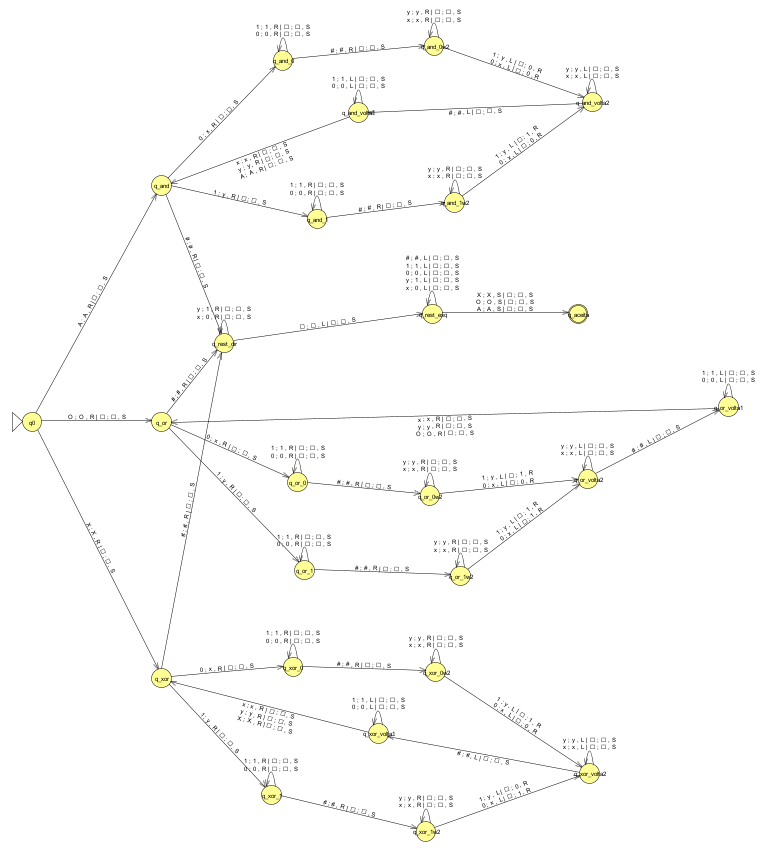
\includegraphics[width=\linewidth,height=0.72\textheight,keepaspectratio]{figuras/diagramas/diag_completo.png}
\caption{Diagrama completo da máquina (25 estados, 89 transições)}
\label{fig:diagrama}
\end{figure}}

\newcommand{\FiguraBlocos}{%
\begin{figure}[H]
\centering
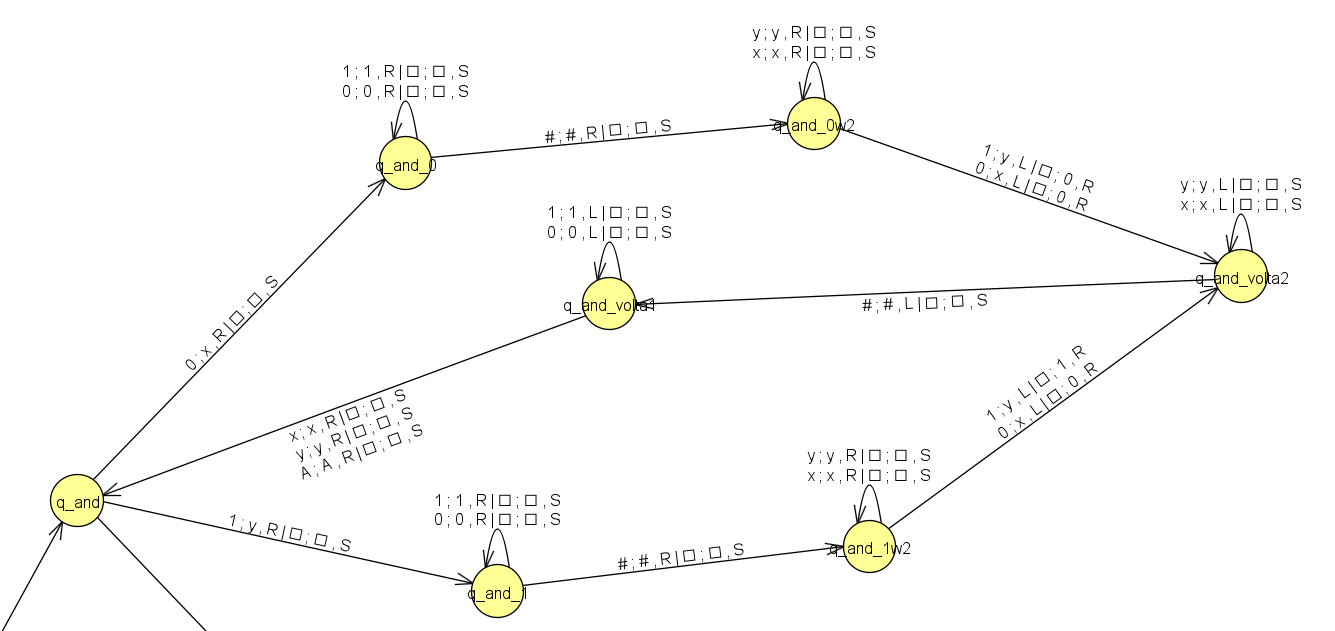
\includegraphics[width=\linewidth,height=0.22\textheight,keepaspectratio]{figuras/diagramas/diag_and.png}\\[0.2em]
{\small (a) Bloco AND}\\[0.8em]
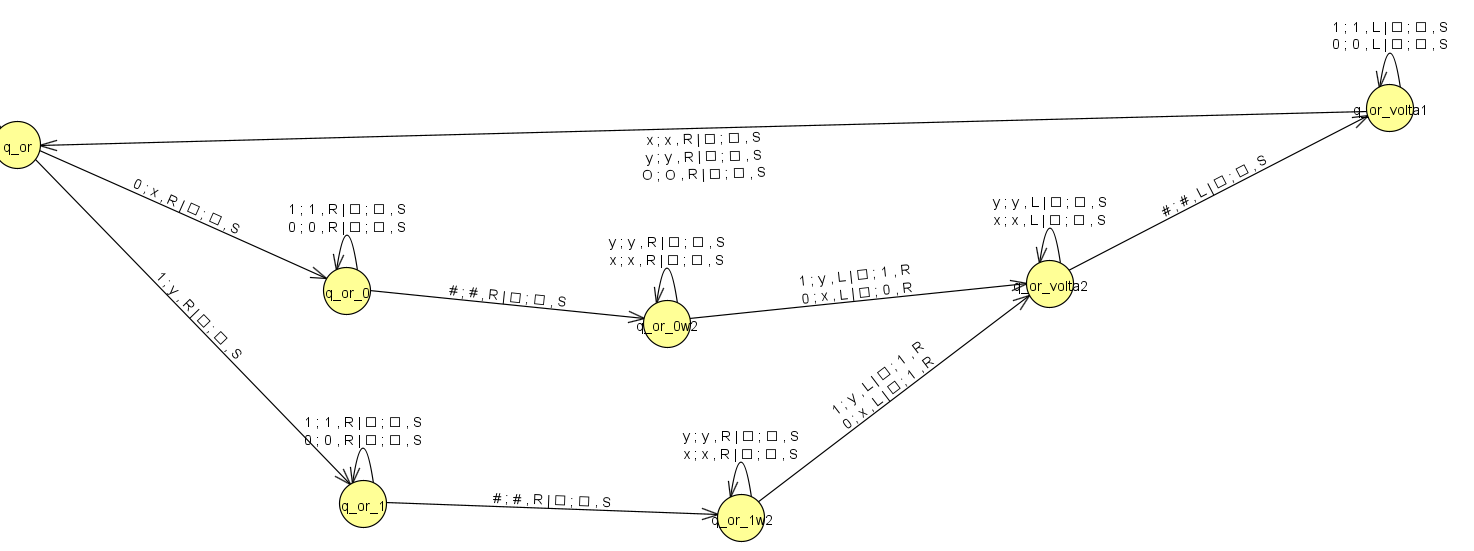
\includegraphics[width=\linewidth,height=0.22\textheight,keepaspectratio]{figuras/diagramas/diag_or.png}\\[0.2em]
{\small (b) Bloco OR}\\[0.8em]
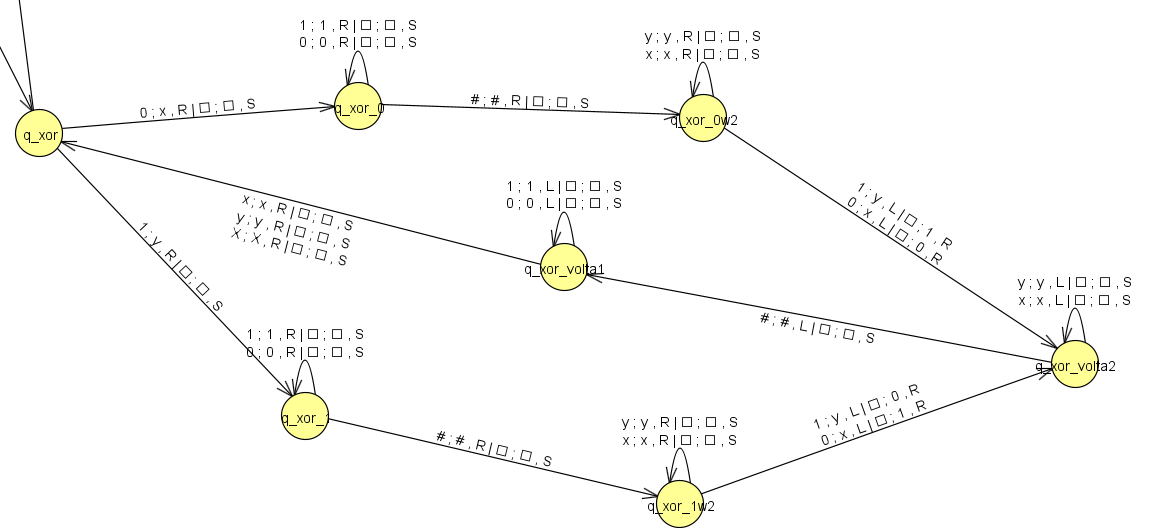
\includegraphics[width=\linewidth,height=0.22\textheight,keepaspectratio]{figuras/diagramas/diag_xor.png}\\[0.2em]
{\small (c) Bloco XOR}
\caption{Ampliação de cada bloco de operação}
\label{fig:blocos}
\end{figure}}

% ======================================================================
% Capítulo 3 -- Resumo dos testes
% ======================================================================

\newcommand{\FiguraResumo}{%
\begin{figure}[H]
\centering
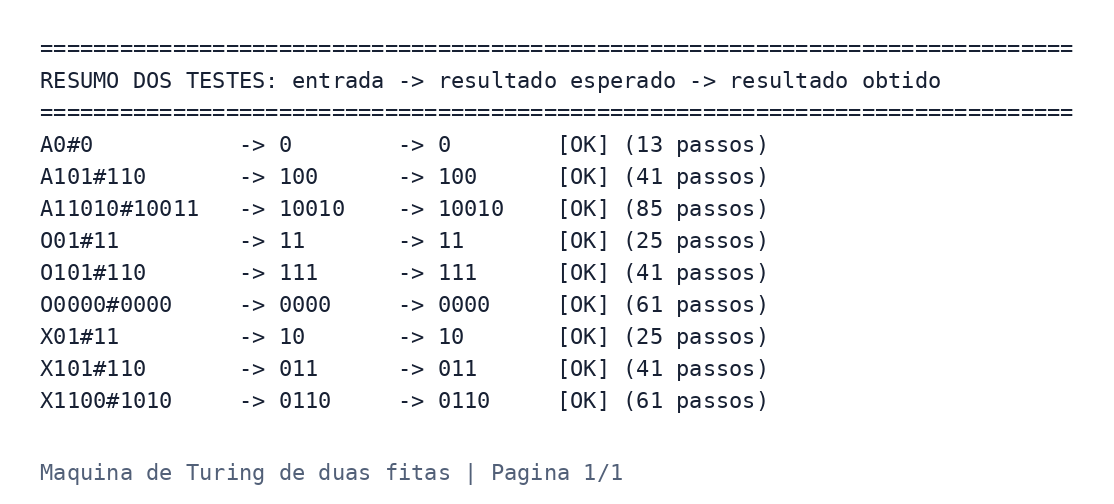
\includegraphics[width=\linewidth]{figuras/resumo.png}
\caption{Resumo da execução dos testes}
\label{fig:resumo}
\end{figure}}

% ======================================================================
% Capítulo 3 -- Execução passo a passo
% ======================================================================

% \PaginaExecucao{arquivo}{entrada}{esperado}{parte}{total}
\newcommand{\PaginaExecucao}[5]{%
\begin{figure}[H]
\centering
\includegraphics[width=\linewidth,height=0.78\textheight,keepaspectratio]{figuras/execucao/#1.png}
\caption{Execução passo a passo da entrada \texttt{#2} (esperado: \texttt{#3})\ifnum#5>1\ --- parte #4 de #5\fi}
\end{figure}}

\newcommand{\FigurasExecucao}{%

% ── Teste 1: A0#0 → 0 (13 passos) ─────────────────────────────────────
\subsection{Teste 1: \texttt{A0\#0}}
\label{sec:teste1}
\PaginaExecucao{teste1_01}{A0\#0}{0}{1}{1}

% ── Teste 2: A101#110 → 100 (41 passos) ───────────────────────────────
\subsection{Teste 2: \texttt{A101\#110}}
\label{sec:teste2}
\PaginaExecucao{teste2_01}{A101\#110}{100}{1}{3}
\PaginaExecucao{teste2_02}{A101\#110}{100}{2}{3}
\PaginaExecucao{teste2_03}{A101\#110}{100}{3}{3}

% ── Teste 3: A11010#10011 → 10010 (85 passos) ─────────────────────────
\subsection{Teste 3: \texttt{A11010\#10011}}
\label{sec:teste3}
\PaginaExecucao{teste3_01}{A11010\#10011}{10010}{1}{6}
\PaginaExecucao{teste3_02}{A11010\#10011}{10010}{2}{6}
\PaginaExecucao{teste3_03}{A11010\#10011}{10010}{3}{6}
\PaginaExecucao{teste3_04}{A11010\#10011}{10010}{4}{6}
\PaginaExecucao{teste3_05}{A11010\#10011}{10010}{5}{6}
\PaginaExecucao{teste3_06}{A11010\#10011}{10010}{6}{6}

% ── Teste 4: O01#11 → 11 (25 passos) ──────────────────────────────────
\subsection{Teste 4: \texttt{O01\#11}}
\label{sec:teste4}
\PaginaExecucao{teste4_01}{O01\#11}{11}{1}{2}
\PaginaExecucao{teste4_02}{O01\#11}{11}{2}{2}

% ── Teste 5: O101#110 → 111 (41 passos) ───────────────────────────────
\subsection{Teste 5: \texttt{O101\#110}}
\label{sec:teste5}
\PaginaExecucao{teste5_01}{O101\#110}{111}{1}{3}
\PaginaExecucao{teste5_02}{O101\#110}{111}{2}{3}
\PaginaExecucao{teste5_03}{O101\#110}{111}{3}{3}

% ── Teste 6: O0000#0000 → 0000 (61 passos) ────────────────────────────
\subsection{Teste 6: \texttt{O0000\#0000}}
\label{sec:teste6}
\PaginaExecucao{teste6_01}{O0000\#0000}{0000}{1}{4}
\PaginaExecucao{teste6_02}{O0000\#0000}{0000}{2}{4}
\PaginaExecucao{teste6_03}{O0000\#0000}{0000}{3}{4}
\PaginaExecucao{teste6_04}{O0000\#0000}{0000}{4}{4}

% ── Teste 7: X01#11 → 10 (25 passos) ──────────────────────────────────
\subsection{Teste 7: \texttt{X01\#11}}
\label{sec:teste7}
\PaginaExecucao{teste7_01}{X01\#11}{10}{1}{2}
\PaginaExecucao{teste7_02}{X01\#11}{10}{2}{2}

% ── Teste 8: X101#110 → 011 (41 passos) ───────────────────────────────
\subsection{Teste 8: \texttt{X101\#110}}
\label{sec:teste8}
\PaginaExecucao{teste8_01}{X101\#110}{011}{1}{3}
\PaginaExecucao{teste8_02}{X101\#110}{011}{2}{3}
\PaginaExecucao{teste8_03}{X101\#110}{011}{3}{3}

% ── Teste 9: X1100#1010 → 0110 (61 passos) ────────────────────────────
\subsection{Teste 9: \texttt{X1100\#1010}}
\label{sec:teste9}
\PaginaExecucao{teste9_01}{X1100\#1010}{0110}{1}{4}
\PaginaExecucao{teste9_02}{X1100\#1010}{0110}{2}{4}
\PaginaExecucao{teste9_03}{X1100\#1010}{0110}{3}{4}
\PaginaExecucao{teste9_04}{X1100\#1010}{0110}{4}{4}
}
).
%%
%% Organização da pasta figuras/:
%%   figuras/diagramas/   diagramas de transição (completo e por bloco)
%%   figuras/resumo.png   tabela final dos 9 testes
%%   figuras/execucao/    passo a passo de cada teste (testeN_PP.png)
%%
%% figuras/resumo.png e figuras/execucao/ foram geradas pelo simulador da
%% pasta MaquinaDeTuring (função salvar_imagens, 48 linhas por página):
%%   python3 mt_duas_fitas.py --resumo --imagem figuras/resumo.png
%% O passo a passo de cada teste (na ordem da lista TESTES) foi salvo sem a
%% tabela de resumo no final, como figuras/execucao/testeN_PP.png.

% ======================================================================
% Capítulo 1 -- Diagramas de transição
% ======================================================================

\newcommand{\FiguraDiagramaCompleto}{%
\begin{figure}[H]
\centering
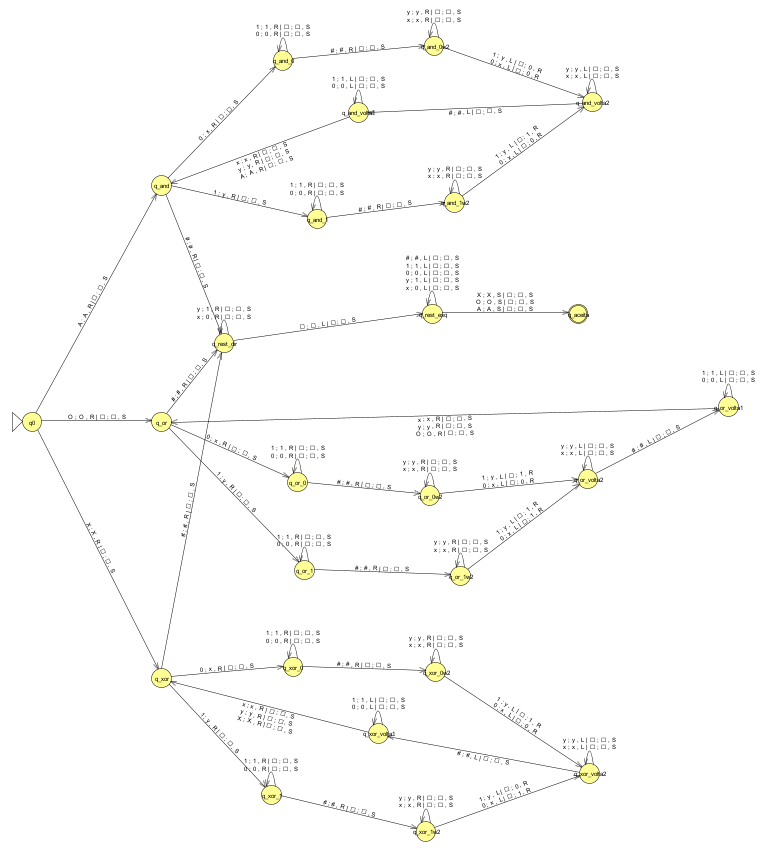
\includegraphics[width=\linewidth,height=0.72\textheight,keepaspectratio]{figuras/diagramas/diag_completo.png}
\caption{Diagrama completo da máquina (25 estados, 89 transições)}
\label{fig:diagrama}
\end{figure}}

\newcommand{\FiguraBlocos}{%
\begin{figure}[H]
\centering
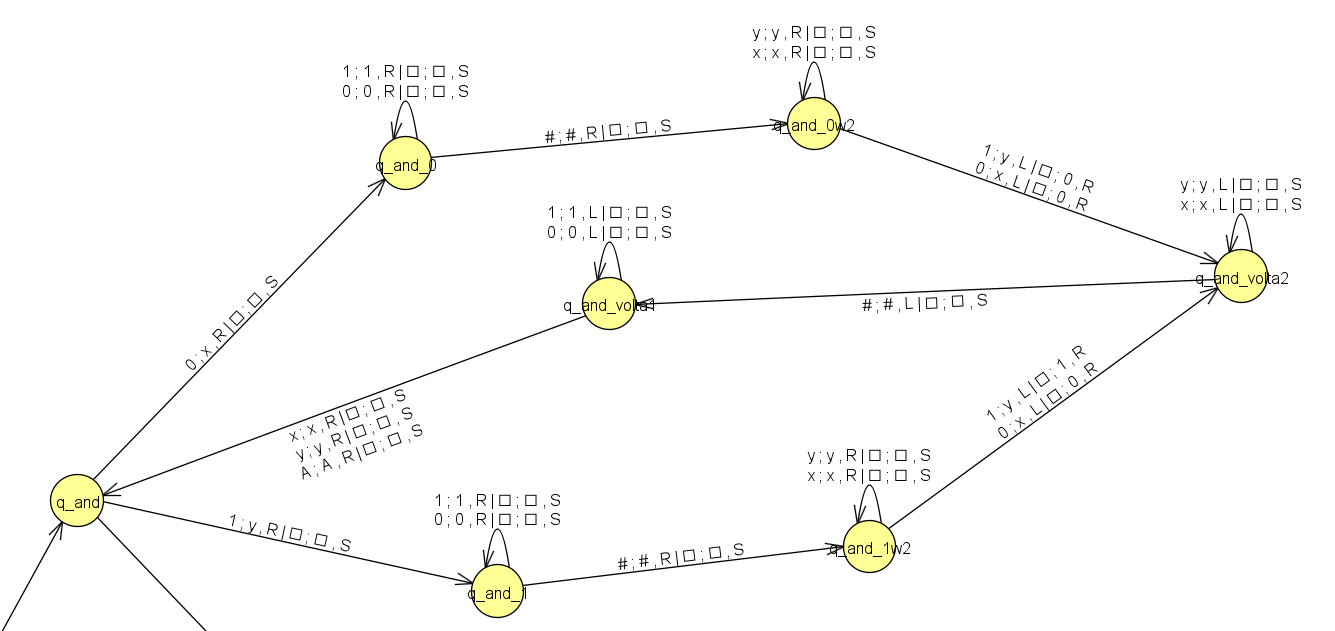
\includegraphics[width=\linewidth,height=0.22\textheight,keepaspectratio]{figuras/diagramas/diag_and.png}\\[0.2em]
{\small (a) Bloco AND}\\[0.8em]
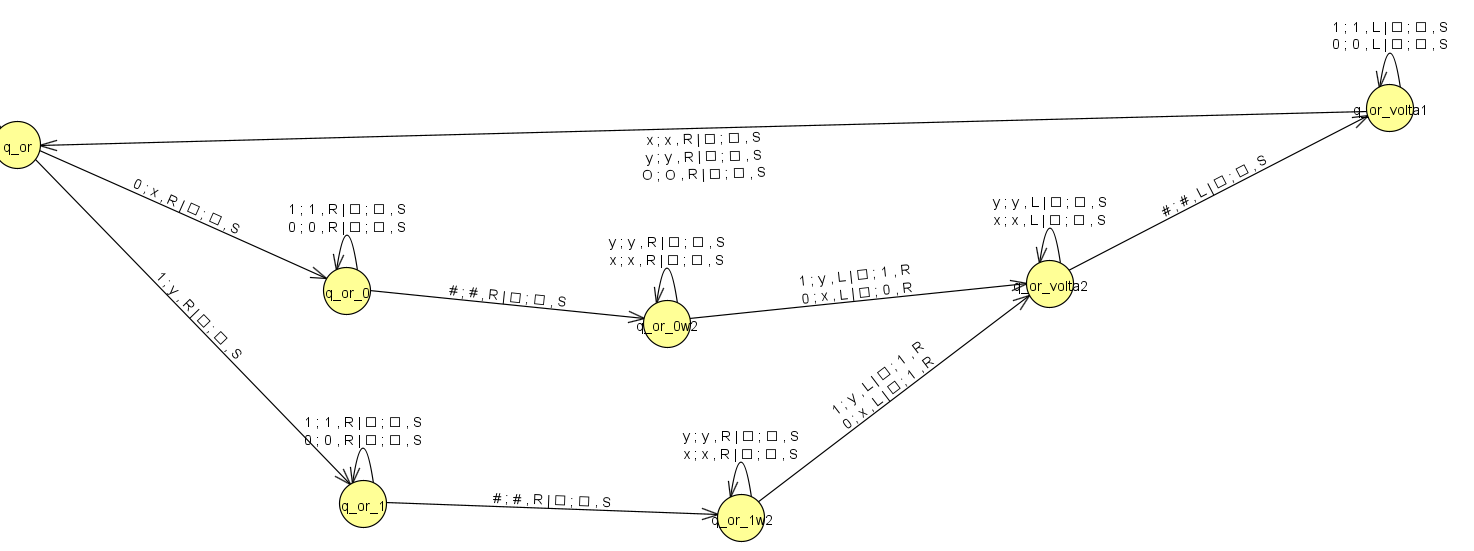
\includegraphics[width=\linewidth,height=0.22\textheight,keepaspectratio]{figuras/diagramas/diag_or.png}\\[0.2em]
{\small (b) Bloco OR}\\[0.8em]
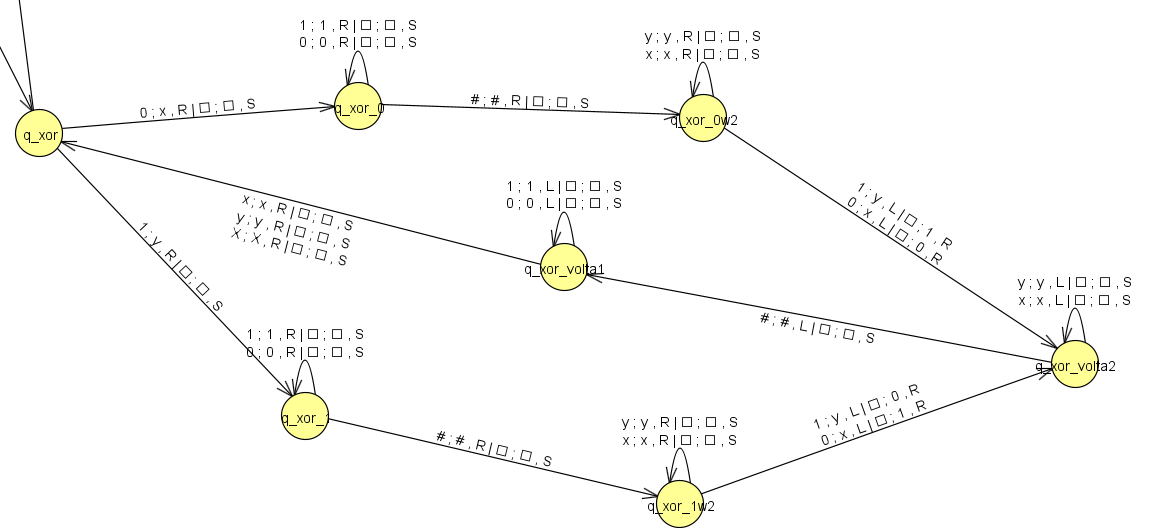
\includegraphics[width=\linewidth,height=0.22\textheight,keepaspectratio]{figuras/diagramas/diag_xor.png}\\[0.2em]
{\small (c) Bloco XOR}
\caption{Ampliação de cada bloco de operação}
\label{fig:blocos}
\end{figure}}

% ======================================================================
% Capítulo 3 -- Resumo dos testes
% ======================================================================

\newcommand{\FiguraResumo}{%
\begin{figure}[H]
\centering
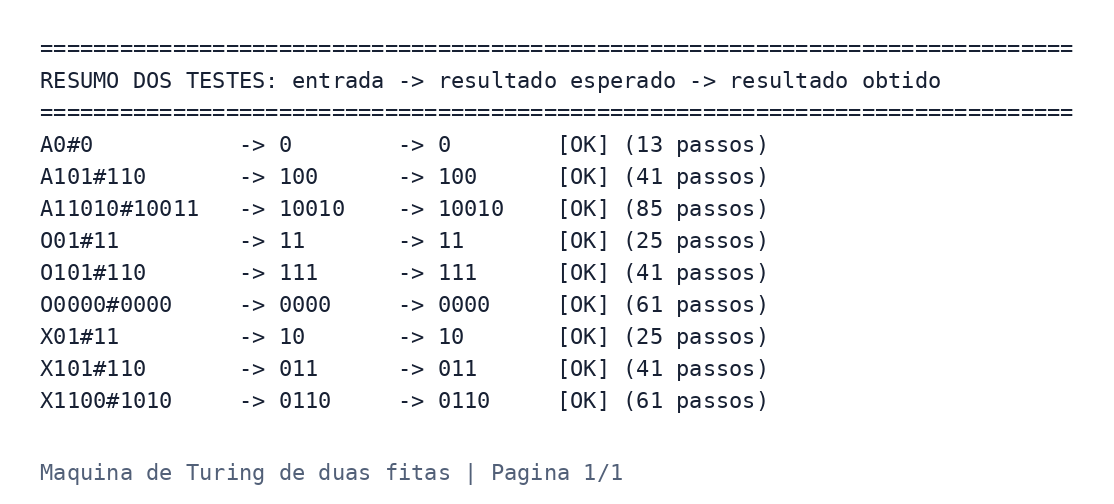
\includegraphics[width=\linewidth]{figuras/resumo.png}
\caption{Resumo da execução dos testes}
\label{fig:resumo}
\end{figure}}

% ======================================================================
% Capítulo 3 -- Execução passo a passo
% ======================================================================

% \PaginaExecucao{arquivo}{entrada}{esperado}{parte}{total}
\newcommand{\PaginaExecucao}[5]{%
\begin{figure}[H]
\centering
\includegraphics[width=\linewidth,height=0.78\textheight,keepaspectratio]{figuras/execucao/#1.png}
\caption{Execução passo a passo da entrada \texttt{#2} (esperado: \texttt{#3})\ifnum#5>1\ --- parte #4 de #5\fi}
\end{figure}}

\newcommand{\FigurasExecucao}{%

% ── Teste 1: A0#0 → 0 (13 passos) ─────────────────────────────────────
\subsection{Teste 1: \texttt{A0\#0}}
\label{sec:teste1}
\PaginaExecucao{teste1_01}{A0\#0}{0}{1}{1}

% ── Teste 2: A101#110 → 100 (41 passos) ───────────────────────────────
\subsection{Teste 2: \texttt{A101\#110}}
\label{sec:teste2}
\PaginaExecucao{teste2_01}{A101\#110}{100}{1}{3}
\PaginaExecucao{teste2_02}{A101\#110}{100}{2}{3}
\PaginaExecucao{teste2_03}{A101\#110}{100}{3}{3}

% ── Teste 3: A11010#10011 → 10010 (85 passos) ─────────────────────────
\subsection{Teste 3: \texttt{A11010\#10011}}
\label{sec:teste3}
\PaginaExecucao{teste3_01}{A11010\#10011}{10010}{1}{6}
\PaginaExecucao{teste3_02}{A11010\#10011}{10010}{2}{6}
\PaginaExecucao{teste3_03}{A11010\#10011}{10010}{3}{6}
\PaginaExecucao{teste3_04}{A11010\#10011}{10010}{4}{6}
\PaginaExecucao{teste3_05}{A11010\#10011}{10010}{5}{6}
\PaginaExecucao{teste3_06}{A11010\#10011}{10010}{6}{6}

% ── Teste 4: O01#11 → 11 (25 passos) ──────────────────────────────────
\subsection{Teste 4: \texttt{O01\#11}}
\label{sec:teste4}
\PaginaExecucao{teste4_01}{O01\#11}{11}{1}{2}
\PaginaExecucao{teste4_02}{O01\#11}{11}{2}{2}

% ── Teste 5: O101#110 → 111 (41 passos) ───────────────────────────────
\subsection{Teste 5: \texttt{O101\#110}}
\label{sec:teste5}
\PaginaExecucao{teste5_01}{O101\#110}{111}{1}{3}
\PaginaExecucao{teste5_02}{O101\#110}{111}{2}{3}
\PaginaExecucao{teste5_03}{O101\#110}{111}{3}{3}

% ── Teste 6: O0000#0000 → 0000 (61 passos) ────────────────────────────
\subsection{Teste 6: \texttt{O0000\#0000}}
\label{sec:teste6}
\PaginaExecucao{teste6_01}{O0000\#0000}{0000}{1}{4}
\PaginaExecucao{teste6_02}{O0000\#0000}{0000}{2}{4}
\PaginaExecucao{teste6_03}{O0000\#0000}{0000}{3}{4}
\PaginaExecucao{teste6_04}{O0000\#0000}{0000}{4}{4}

% ── Teste 7: X01#11 → 10 (25 passos) ──────────────────────────────────
\subsection{Teste 7: \texttt{X01\#11}}
\label{sec:teste7}
\PaginaExecucao{teste7_01}{X01\#11}{10}{1}{2}
\PaginaExecucao{teste7_02}{X01\#11}{10}{2}{2}

% ── Teste 8: X101#110 → 011 (41 passos) ───────────────────────────────
\subsection{Teste 8: \texttt{X101\#110}}
\label{sec:teste8}
\PaginaExecucao{teste8_01}{X101\#110}{011}{1}{3}
\PaginaExecucao{teste8_02}{X101\#110}{011}{2}{3}
\PaginaExecucao{teste8_03}{X101\#110}{011}{3}{3}

% ── Teste 9: X1100#1010 → 0110 (61 passos) ────────────────────────────
\subsection{Teste 9: \texttt{X1100\#1010}}
\label{sec:teste9}
\PaginaExecucao{teste9_01}{X1100\#1010}{0110}{1}{4}
\PaginaExecucao{teste9_02}{X1100\#1010}{0110}{2}{4}
\PaginaExecucao{teste9_03}{X1100\#1010}{0110}{3}{4}
\PaginaExecucao{teste9_04}{X1100\#1010}{0110}{4}{4}
}
).
%%
%% Organização da pasta figuras/:
%%   figuras/diagramas/   diagramas de transição (completo e por bloco)
%%   figuras/resumo.png   tabela final dos 9 testes
%%   figuras/execucao/    passo a passo de cada teste (testeN_PP.png)
%%
%% figuras/resumo.png e figuras/execucao/ foram geradas pelo simulador da
%% pasta MaquinaDeTuring (função salvar_imagens, 48 linhas por página):
%%   python3 mt_duas_fitas.py --resumo --imagem figuras/resumo.png
%% O passo a passo de cada teste (na ordem da lista TESTES) foi salvo sem a
%% tabela de resumo no final, como figuras/execucao/testeN_PP.png.

% ======================================================================
% Capítulo 1 -- Diagramas de transição
% ======================================================================

\newcommand{\FiguraDiagramaCompleto}{%
\begin{figure}[H]
\centering
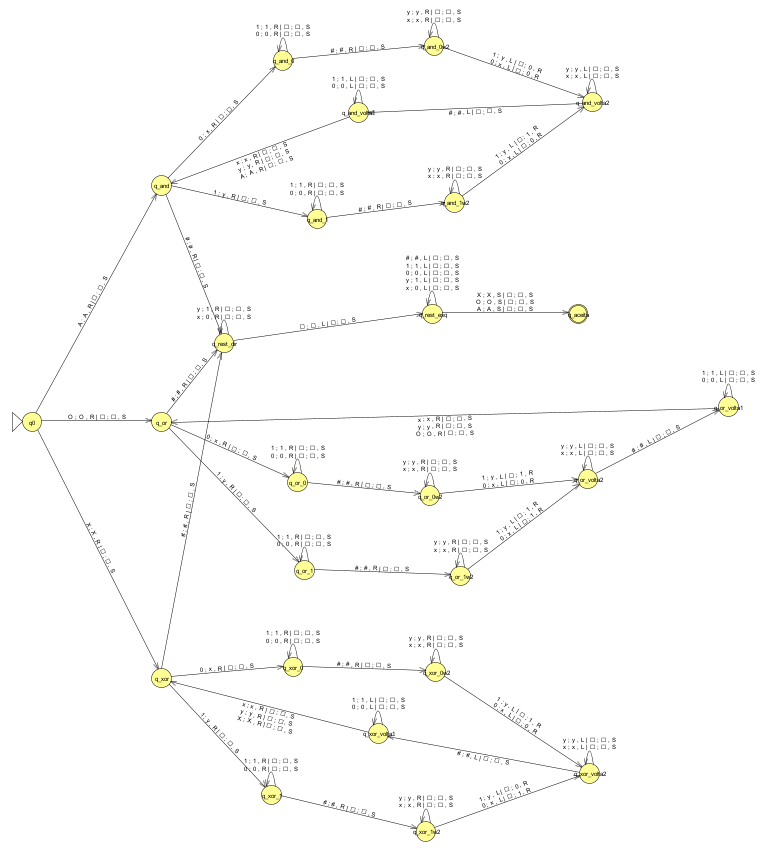
\includegraphics[width=\linewidth,height=0.72\textheight,keepaspectratio]{figuras/diagramas/diag_completo.png}
\caption{Diagrama completo da máquina (25 estados, 89 transições)}
\label{fig:diagrama}
\end{figure}}

\newcommand{\FiguraBlocos}{%
\begin{figure}[H]
\centering
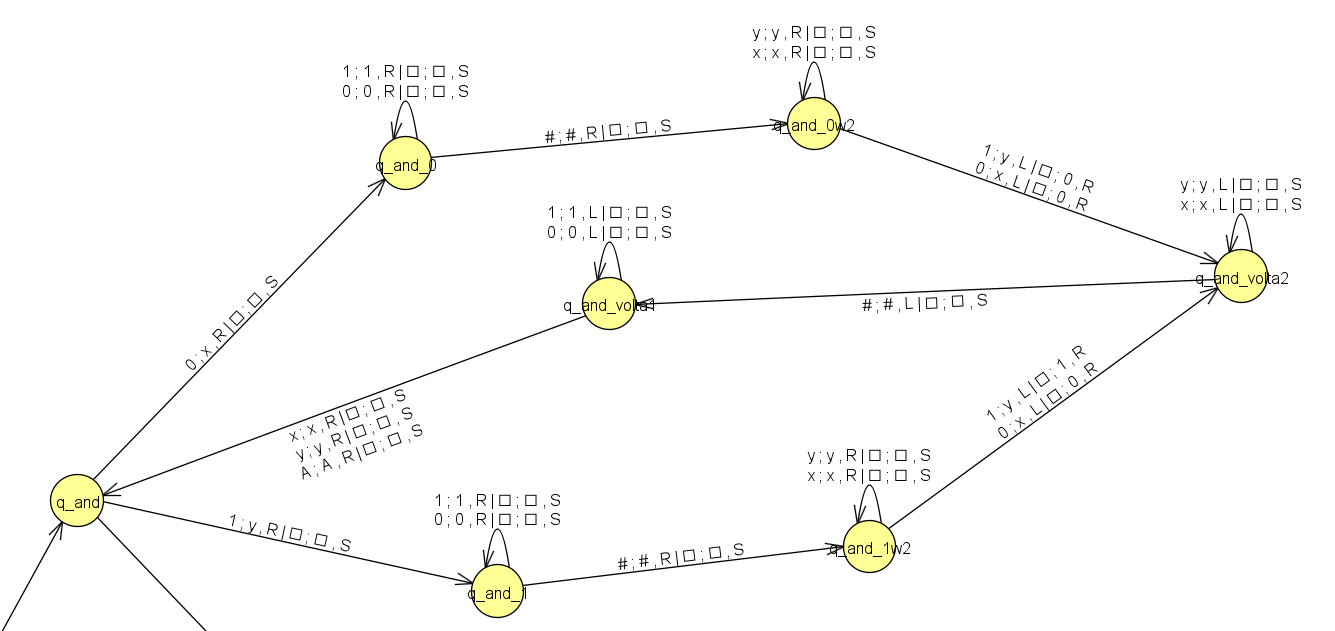
\includegraphics[width=\linewidth,height=0.22\textheight,keepaspectratio]{figuras/diagramas/diag_and.png}\\[0.2em]
{\small (a) Bloco AND}\\[0.8em]
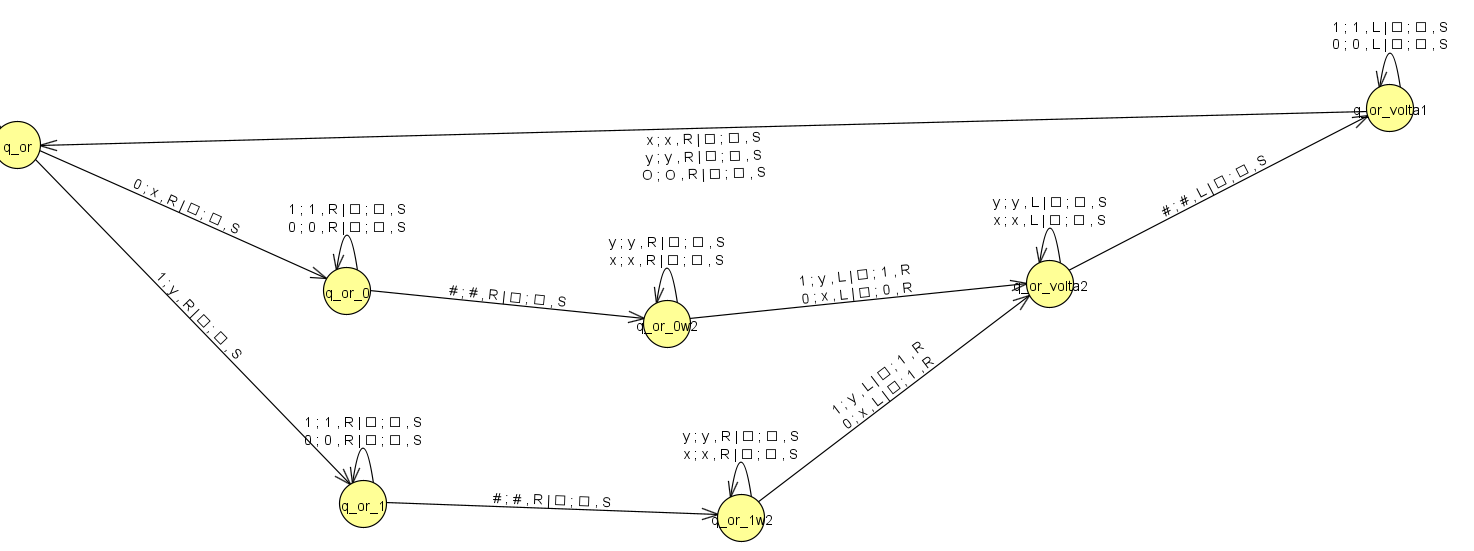
\includegraphics[width=\linewidth,height=0.22\textheight,keepaspectratio]{figuras/diagramas/diag_or.png}\\[0.2em]
{\small (b) Bloco OR}\\[0.8em]
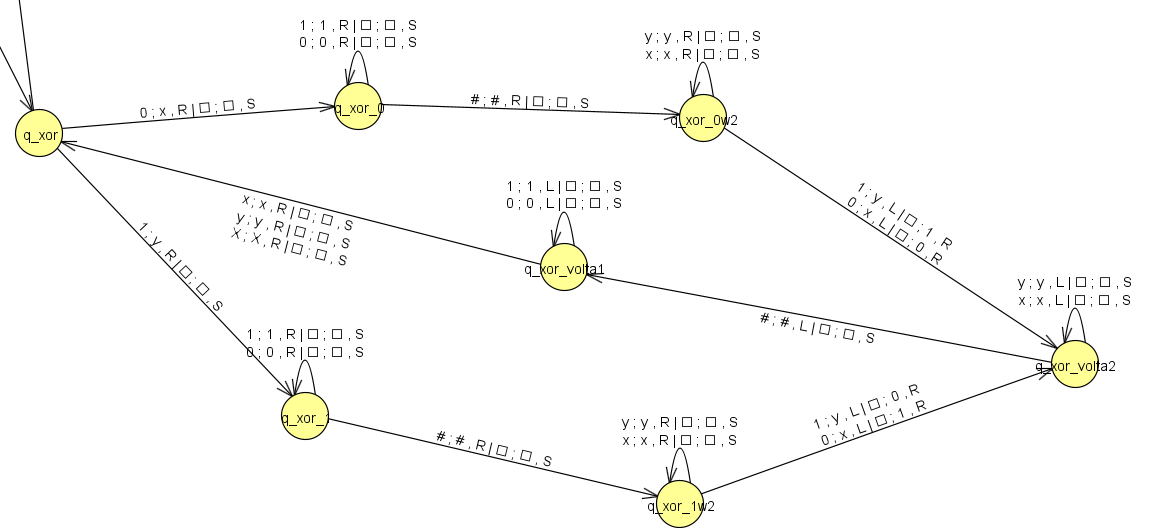
\includegraphics[width=\linewidth,height=0.22\textheight,keepaspectratio]{figuras/diagramas/diag_xor.png}\\[0.2em]
{\small (c) Bloco XOR}
\caption{Ampliação de cada bloco de operação}
\label{fig:blocos}
\end{figure}}

% ======================================================================
% Capítulo 3 -- Resumo dos testes
% ======================================================================

\newcommand{\FiguraResumo}{%
\begin{figure}[H]
\centering
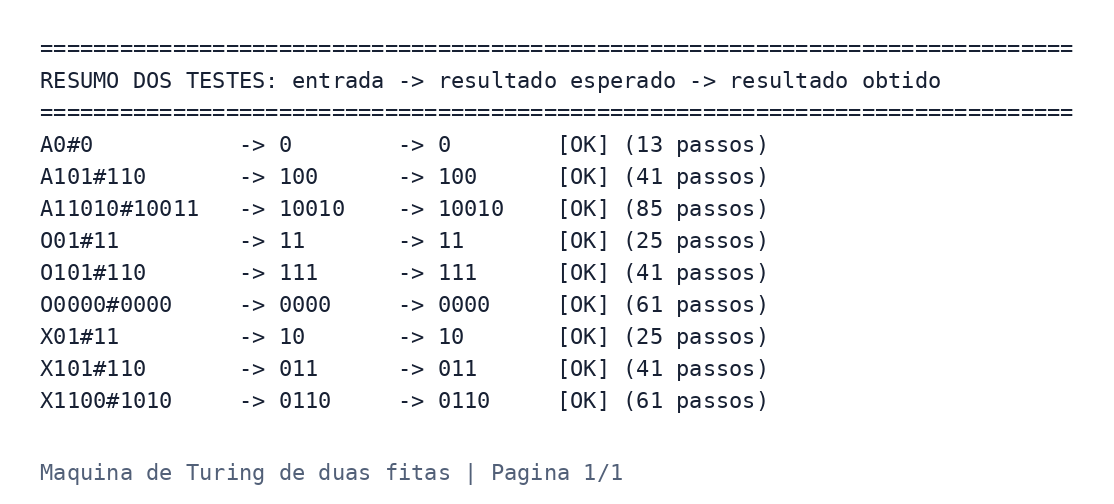
\includegraphics[width=\linewidth]{figuras/resumo.png}
\caption{Resumo da execução dos testes}
\label{fig:resumo}
\end{figure}}

% ======================================================================
% Capítulo 3 -- Execução passo a passo
% ======================================================================

% \PaginaExecucao{arquivo}{entrada}{esperado}{parte}{total}
\newcommand{\PaginaExecucao}[5]{%
\begin{figure}[H]
\centering
\includegraphics[width=\linewidth,height=0.78\textheight,keepaspectratio]{figuras/execucao/#1.png}
\caption{Execução passo a passo da entrada \texttt{#2} (esperado: \texttt{#3})\ifnum#5>1\ --- parte #4 de #5\fi}
\end{figure}}

\newcommand{\FigurasExecucao}{%

% ── Teste 1: A0#0 → 0 (13 passos) ─────────────────────────────────────
\subsection{Teste 1: \texttt{A0\#0}}
\label{sec:teste1}
\PaginaExecucao{teste1_01}{A0\#0}{0}{1}{1}

% ── Teste 2: A101#110 → 100 (41 passos) ───────────────────────────────
\subsection{Teste 2: \texttt{A101\#110}}
\label{sec:teste2}
\PaginaExecucao{teste2_01}{A101\#110}{100}{1}{3}
\PaginaExecucao{teste2_02}{A101\#110}{100}{2}{3}
\PaginaExecucao{teste2_03}{A101\#110}{100}{3}{3}

% ── Teste 3: A11010#10011 → 10010 (85 passos) ─────────────────────────
\subsection{Teste 3: \texttt{A11010\#10011}}
\label{sec:teste3}
\PaginaExecucao{teste3_01}{A11010\#10011}{10010}{1}{6}
\PaginaExecucao{teste3_02}{A11010\#10011}{10010}{2}{6}
\PaginaExecucao{teste3_03}{A11010\#10011}{10010}{3}{6}
\PaginaExecucao{teste3_04}{A11010\#10011}{10010}{4}{6}
\PaginaExecucao{teste3_05}{A11010\#10011}{10010}{5}{6}
\PaginaExecucao{teste3_06}{A11010\#10011}{10010}{6}{6}

% ── Teste 4: O01#11 → 11 (25 passos) ──────────────────────────────────
\subsection{Teste 4: \texttt{O01\#11}}
\label{sec:teste4}
\PaginaExecucao{teste4_01}{O01\#11}{11}{1}{2}
\PaginaExecucao{teste4_02}{O01\#11}{11}{2}{2}

% ── Teste 5: O101#110 → 111 (41 passos) ───────────────────────────────
\subsection{Teste 5: \texttt{O101\#110}}
\label{sec:teste5}
\PaginaExecucao{teste5_01}{O101\#110}{111}{1}{3}
\PaginaExecucao{teste5_02}{O101\#110}{111}{2}{3}
\PaginaExecucao{teste5_03}{O101\#110}{111}{3}{3}

% ── Teste 6: O0000#0000 → 0000 (61 passos) ────────────────────────────
\subsection{Teste 6: \texttt{O0000\#0000}}
\label{sec:teste6}
\PaginaExecucao{teste6_01}{O0000\#0000}{0000}{1}{4}
\PaginaExecucao{teste6_02}{O0000\#0000}{0000}{2}{4}
\PaginaExecucao{teste6_03}{O0000\#0000}{0000}{3}{4}
\PaginaExecucao{teste6_04}{O0000\#0000}{0000}{4}{4}

% ── Teste 7: X01#11 → 10 (25 passos) ──────────────────────────────────
\subsection{Teste 7: \texttt{X01\#11}}
\label{sec:teste7}
\PaginaExecucao{teste7_01}{X01\#11}{10}{1}{2}
\PaginaExecucao{teste7_02}{X01\#11}{10}{2}{2}

% ── Teste 8: X101#110 → 011 (41 passos) ───────────────────────────────
\subsection{Teste 8: \texttt{X101\#110}}
\label{sec:teste8}
\PaginaExecucao{teste8_01}{X101\#110}{011}{1}{3}
\PaginaExecucao{teste8_02}{X101\#110}{011}{2}{3}
\PaginaExecucao{teste8_03}{X101\#110}{011}{3}{3}

% ── Teste 9: X1100#1010 → 0110 (61 passos) ────────────────────────────
\subsection{Teste 9: \texttt{X1100\#1010}}
\label{sec:teste9}
\PaginaExecucao{teste9_01}{X1100\#1010}{0110}{1}{4}
\PaginaExecucao{teste9_02}{X1100\#1010}{0110}{2}{4}
\PaginaExecucao{teste9_03}{X1100\#1010}{0110}{3}{4}
\PaginaExecucao{teste9_04}{X1100\#1010}{0110}{4}{4}
}
